\documentclass[11pt]{article}

\usepackage[T1]{fontenc}
\usepackage[utf8]{inputenc}
\usepackage{lmodern}
\usepackage[margin=1in]{geometry}
\usepackage{amsmath,amssymb}
\usepackage{booktabs}
\usepackage{tabularx}
\usepackage{array}
\usepackage[final]{graphicx}
\usepackage{float}
\usepackage{enumitem}
\usepackage{microtype}
\usepackage{xurl}
\usepackage[hidelinks]{hyperref}
\hypersetup{
  pdftitle={Predicting NBA Player-Game Field-Goal Attempts, Rebound Chances, and Rebounds with Similar-Player Matchups and Residual Learning},
  pdfauthor={Malachi Fordham},
  pdfsubject={NBA player-game opportunity forecasting},
  pdfkeywords={NBA analytics, player tracking, Elastic Net, residual learning, matchup modeling}
}
\graphicspath{{figures/}}
\setkeys{Gin}{draft=false}
\setlist{nosep}
\setlength{\emergencystretch}{3em}

\newcommand{\RC}{\mathrm{RC}}
\newcommand{\Vone}{\mathrm{V1}}
\newcommand{\Vtwo}{\mathrm{V2}}

\title{Predicting NBA Player-Game Field-Goal Attempts, Rebound Chances, and Rebounds\\
with Similar-Player Matchups and Residual Learning}
\author{Malachi Fordham}
\date{August 2026}

\begin{document}

\maketitle

\begin{abstract}
This study develops and evaluates a pregame model for NBA player field-goal
attempts (FGA), rebound chances (RC), and rebounds (REB). The approach separates
opportunity from conversion. An interpretable first-stage model estimates a player's recent stable workload,
identifies statistically similar players, and uses the comparable players'
per-minute results against the same opponent to estimate an opponent effect.
After sample-size shrinkage and bounding, that effect is applied to the
target player's recent per-game opportunity baseline. A second
stage uses Elastic Net regression to learn residual errors left by this
basketball baseline; rebounds are then obtained from corrected rebound chances
and a separately learned rebound-conversion adjustment.

The study uses NBA regular-season player-game data from 2021--22 through
2025--26 and evaluates model choices with chronological, rolling outer-season
tests. Across the 2023--24, 2024--25, and 2025--26 chronologically held-out test seasons, the selected
opportunity model reduced equal-season mean absolute error by 2.36\% for FGA,
4.22\% for rebound chances, and 2.64\% for rebounds relative to the tuned
first-stage baseline. The learned conversion layer reduced rebound error by a
further 0.86\% across complete held-out seasons. A model trained only on
normal-minute games modestly improved conditional FGA and rebound-chance
accuracy. The final system selects Elastic Net over a competitive neural benchmark
because it achieved nearly equal accuracy while remaining easier to interpret
and substantially faster to fit.
\end{abstract}

\section{Introduction}

Single-game NBA box-score outcomes combine several mechanisms. A player's
field-goal attempts and rebound chances depend on workload and role, while
actual rebounds also depend on how efficiently available chances are
converted. Treating each result as one indivisible target obscures this
structure.

For target player $p$, opponent $o$, and game date $d$, this project estimates

\[
\widehat{FGA}_{p,o,d}, \qquad
\widehat{\RC}_{p,o,d}, \qquad
\widehat{REB}_{p,o,d},
\]

using only information available before tip-off. The design began as an
interpretable comparison model: establish the target's recent baseline, find
players whose current workload and playing style are similar, measure how
their opportunity changed against the target opponent, and transfer a
carefully weighted portion of that effect to the target. Machine learning was
added only after this rule-based model was complete, allowing the learned
component to correct systematic errors without discarding the underlying
basketball interpretation.
\newpage
The study makes four practical contributions:

\begin{enumerate}
    \item a reproducible definition of player similarity based on workload,
    opportunity, involvement, listed position, and starting role;
    \item an interpretable opponent adjustment with explicit sample-size trust
    and robust bounds;
    \item a leakage-controlled residual-learning framework evaluated on future
    seasons; and
    \item separate all-games and normal-minutes final fitted models, with a
    learned rebound-conversion component.
\end{enumerate}

\section{Research Hypotheses}

The study examines five hypotheses. H3--H5 are evaluated through direct
chronological model comparisons. H1 and H2 are design hypotheses supported by
component behavior, but their isolated effects were not measured in the final
outer-season experiment.

\begin{description}[style=nextline,leftmargin=0pt]
    \item[H1.] A player's recent performance in games with a stable workload
    provides a useful baseline for predicting FGA, rebound chances, and
    rebounds.
    \item[H2.] Opponent-specific per-minute rates from statistically similar
    players improve the target baseline when the evidence is adjusted for
    sample size.
    \item[H3.] Machine-learning models can improve accuracy by learning
    systematic residual errors left by the baseline.
    \item[H4.] Training on games in which players received approximately their
    expected minutes improves predictions conditional on the player receiving
    a normal workload.
    \item[H5.] Modeling rebound conversion separately from rebound opportunity
    improves rebound predictions over using only the player's recent
    conversion rate.
\end{description}

For rebounds,

\[
\widehat{REB}=\widehat{\RC}\times
\widehat{ConversionRate}.
\]

Per-minute rates are used to compare players with different workloads and to
estimate opponent effects among similar players. Final V1 opportunity
predictions apply those effects to the target player's mean qualifying
per-game FGA and rebound-chance baselines. Mean qualifying minutes are retained
as a workload estimate and model feature, but V1 does not explicitly rescale
the final prediction by projected minutes.

Listed position was initially considered as a hard comparison rule. Manual
review showed that basketball role does not always follow position labels, so
the final method uses position as a soft penalty within a broader statistical
profile. This permits cross-position comparisons when workload, usage,
touches, shooting volume, and rebounding opportunity are otherwise similar.

\section{Data}

\subsection{Sources and unit of analysis}

Data were obtained from NBA Stats through the community-maintained
\texttt{nba\_api} Python package \cite{nbaapi}. A canonical warehouse joins
regular-season base box scores, advanced usage statistics, and player tracking
statistics. Each row represents one player appearance in one game and includes
the game date, teams, minutes, FGA, rebounds, rebound chances, touches, usage,
listed position, and starter status.

NBA Stats defines a rebound chance as an event in which a player becomes the
closest player to the ball at some point after the ball descends below the rim
and before the rebound is secured \cite{nbaglossary}. The warehouse stores this
measure from the \texttt{reboundChancesTotal} tracking field.

\subsection{Historical coverage}

The local warehouse covers five complete regular seasons and 131,279
player-game rows.

\begin{table}[H]
\centering
\caption{Canonical historical warehouse.}
\label{tab:warehouse}
\small
\begin{tabular}{lrrrr}
\toprule
Season & Games & Players & Player-games & Tracking/usage coverage \\
\midrule
2021--22 & 1,230 & 605 & 26,036 & 100\% \\
2022--23 & 1,230 & 539 & 25,892 & 100\% \\
2023--24 & 1,230 & 572 & 26,399 & 100\% \\
2024--25 & 1,230 & 569 & 26,303 & 100\% \\
2025--26 & 1,230 & 582 & 26,649 & 100\% \\
\bottomrule
\end{tabular}
\end{table}

The finalized 250-player all-games modeling dataset contains 59,156 eligible
target player-games across 5,788 distinct NBA games. Its dates run from October
29, 2021 through April 12, 2026. The first days of a season are often
ineligible because the player has not yet accumulated the required pregame
history.

\subsection{Data quality and leakage controls}

The data pipeline validates required columns, nonnegative statistics, one row
per \texttt{(game\_id, player\_id)}, valid dates, and the expected season for
each partition.

For every modeled game, the feature cutoff is the previous calendar day.
Rolling baselines, player profiles, opponent rates, hyperparameter selection,
and percentile bounds are all constructed from earlier data. Actual outcomes
are attached only after pregame features are complete. The normal-minutes label
uses actual game minutes solely to define research cohorts; it is never an
inference feature.

\section{Methodology}

\subsection{Recent target baseline}

For a target game on date $d$, the model uses the 30 days ending at $d-1$.
Let $M_i$ be minutes in each recent appearance. The initial workload estimate
and qualification threshold are

\[
M_{usual}=\operatorname{mean}(M_i), \qquad
M_{min}=0.75M_{usual}.
\]

Games are retained when minutes are at least $M_{min}$
and FGA and rebounds are observed. At least five qualifying box-score games
and five qualifying games with rebound-chance tracking are required.

The baseline records mean qualifying per-game FGA and rebound chances,
corresponding per-minute rates, mean qualifying minutes, and recent rebound
conversion. The
conversion estimate uses paired totals:

\[
Conversion_{recent}=
\frac{\sum_i REB_i}{\sum_i \RC_i}.
\]

Using totals gives high-opportunity games more influence than an unweighted
mean of game-level conversion percentages.

\subsection{Player profiles and similarity}

Each recent player profile contains minutes, FGA per minute, rebound chances
per minute, usage rate, touches per minute, starter rate, starter flag, and
listed position. Numeric features are standardized across eligible players:

\[
z_{ij}=\frac{x_{ij}-\mu_j}{\sigma_j}.
\]

For target $t$ and candidate $i$, weighted numeric distance is

\[
D_{numeric}(i,t)=
\sqrt{
\frac{\sum_j w_j(z_{ij}-z_{tj})^2}
     {\sum_j w_j}
}.
\]

Broad guard, forward, and center tokens are derived from listed position. A
candidate with no token overlap receives a default position penalty of 0.35:

\[
D_{final}=D_{numeric}+PositionPenalty.
\]

Lower distance indicates greater similarity. The target is excluded from the
candidate pool, and the default workflow selects up to ten closest eligible
players. Candidates must have complete recent profiles and valid FGA/minute
and rebound-chances/minute observations against the exact target opponent
within the same lookback window. Default distance weights are reported in
Appendix~\ref{app:parameters}.

\subsection{Opponent evidence, trust, and robust bounds}

For comparable player $s$, metric $m$, and opponent $o$, the matchup ratio is

\[
R_{s,m,o}=\frac{rate_{s,m\;versus\;o}}{rate_{s,m\;overall}}.
\]

Player ratios are combined using the number of valid opponent-game
observations as weights:

\[
R_{raw,m,o}=
\frac{\sum_s n_{s,m,o}R_{s,m,o}}
     {\sum_s n_{s,m,o}}.
\]

FGA and rebound chances retain separate sample counts. Before trust is
applied, the raw multiplier is clipped to a robust interval:

\[
R_{bounded}=\min(1.50,\max(0.50,R_{raw})).
\]

Sample trust follows a piecewise smoothstep curve. The final anchors are
0.45 trust at five samples, 0.65 at ten, and 0.90 at fifteen or more. Within
each interval, interpolation uses

\[
S(x)=x^2(3-2x), \qquad 0\leq x\leq1.
\]

The effective multiplier is a convex combination of observed evidence and the
neutral prior:

\[
R_{effective}=1+w(R_{bounded}-1).
\]

Here, $w$ is the metric-specific sample-trust weight and $1.00$ represents no
opponent adjustment. With little evidence, the effective multiplier remains
close to $1.00$; as the valid sample grows, it moves toward the observed
bounded ratio.

\subsection{Interpretable V1 projection}

The first-stage model predicts

\[
\widehat{FGA}_{\Vone}=FGA_{baseline}\times R_{effective,FGA},
\]

\[
\widehat{\RC}_{\Vone}=\RC_{baseline}\times R_{effective,\RC},
\]

\[
\widehat{REB}_{\Vone}=\widehat{\RC}_{\Vone}
\times Conversion_{recent}.
\]

This model is independently usable and remains the reference prediction that
the machine-learning stage attempts to improve.

\subsection{V2 residual learning}

Rather than replace the interpretable model, V2 predicts its historical error:

\[
Residual_m=Actual_m-\widehat{m}_{\Vone},
\]

\[
\widehat{m}_{\Vtwo}=\max(0,
\widehat{m}_{\Vone}+\widehat{Residual}_m).
\]

Separate models correct FGA and rebound-chance residuals. Features summarize
baseline quality, target role, comparison-pool quality, matchup evidence, and
the V1 projections. The final opportunity schema contains 38 numeric features
and one categorical listed-position feature. The feature groups are summarized
in Appendix~\ref{app:parameters}; the complete machine-readable schema is
defined in the source code and recorded in locally generated model manifests.

Elastic Net combines $L_1$ and $L_2$ regularization \cite{zouhastie} and is
implemented with scikit-learn \cite{scikitlearn}. Median imputation, numeric
standardization, and one-hot position encoding are fitted within each training
period.

\subsection{Learned rebound conversion}

After rebound-chance correction, conversion is modeled separately. For a row
with positive actual rebound chances, the observed conversion target is

\[
C_{actual}=\operatorname{clip}\left(
\frac{REB_{actual}}{\RC_{actual}},0,1\right),
\]

and the learned target is the residual from the recent player rate:

\[
\Delta C=C_{actual}-C_{recent}.
\]

A position-prior alternative was also evaluated:

\[
C_{shrunk}=\frac{E_{recent}C_{recent}+\lambda C_{position}}
{E_{recent}+\lambda},
\]

where $E_{recent}$ is the target's recent paired rebound-chance exposure and
$\lambda$ controls prior strength. The Elastic Net model predicts $\Delta C$.
Training rows are weighted by actual rebound chances so that high-opportunity
games contribute more conversion information. Zero-chance rows are excluded
from conversion fitting but remain in final rebound evaluation. The resulting
conversion rate is clipped to the training period's first and 99th percentile
bounds before final rebounds are calculated:

\[
\widehat{REB}=\widehat{\RC}_{\Vtwo}
\times \widehat{ConversionRate}.
\]

Trust-dependent fields are omitted from conversion features so that changing
the final trust curve does not silently redefine the conversion model.

\begin{figure}[htbp]
\centering
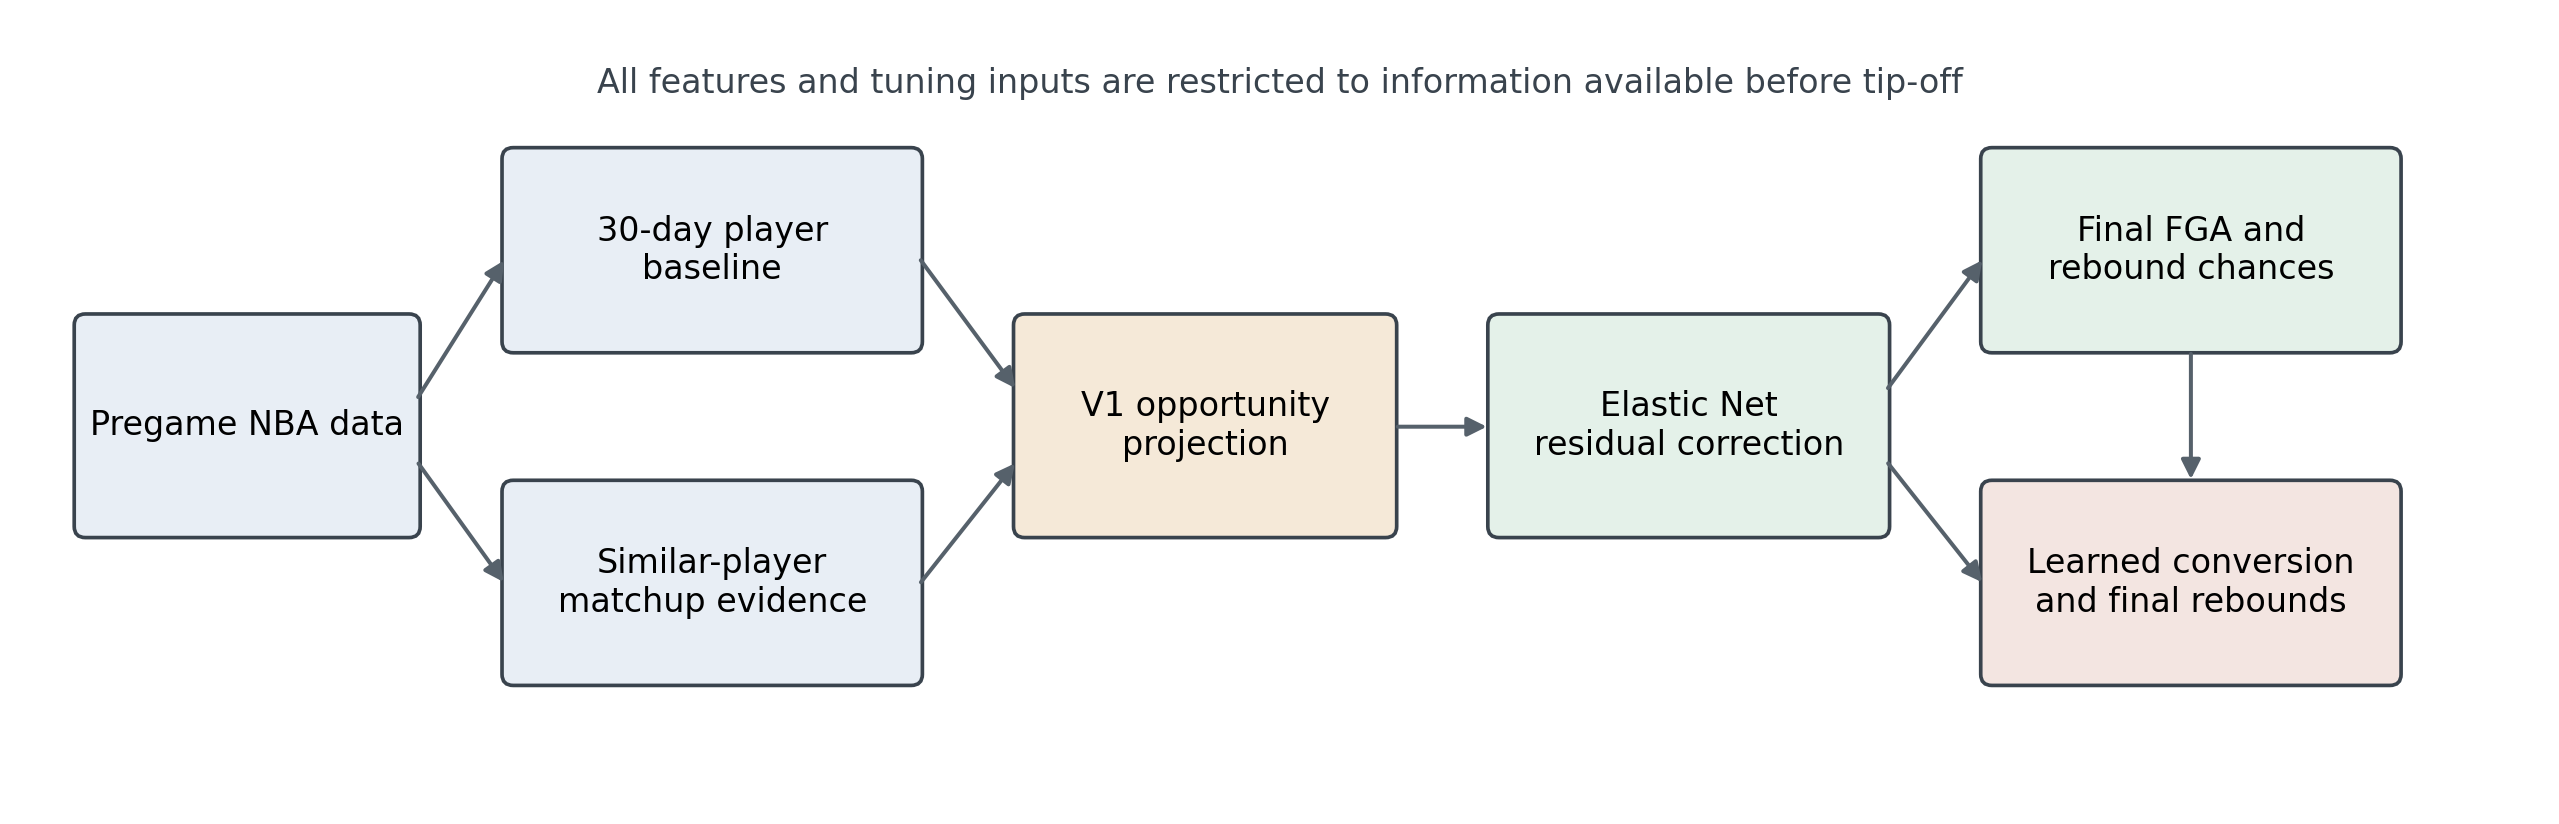
\includegraphics[draft=false,width=\textwidth]{model_pipeline.png}
\caption{Final modeling pipeline. Opportunity and conversion are estimated
separately, and every input is restricted to pregame information.}
\label{fig:pipeline}
\end{figure}

\section{Experimental Design}

\subsection{Reproducible target-player pools}

Convenience samples of well-known players would overrepresent particular
roles. Eligible player-seasons therefore required at least 30 appearances, 20
average minutes, a 50\% starter rate, at least 95\% coverage for usage,
tracking, and starter information, and known usage and broad position.

Players were stratified by broad position and low, medium, or high usage.
Nested pools of 30, 60, 90, 150, and 250 target players were constructed with
seed 42. The target pool determines which player-games become training rows;
similar-player searches still use the full eligible league population
available before each target game.

The eligible universe used to freeze the target pool was constructed from
2021--22 through 2023--24. Consequently, the 2023--24 fold is chronological
with respect to feature construction and model fitting, but its target-cohort
selection was informed by participation and role data from that season.

\subsection{Compared model families}

Three residual model families were evaluated:

\begin{itemize}
    \item \textbf{Elastic Net}: regularized linear residual models with scaled
    numeric features and one-hot position;
    \item \textbf{Histogram Gradient Boosting}: nonlinear tree models using
    median imputation and absolute-error loss; and
    \item \textbf{Multitask multilayer perceptron (MLP)}: a shared 64-to-32
hidden representation with separate FGA and rebound-chance output heads,
implemented in PyTorch \cite{pytorch}. Training used Huber loss, AdamW,
early stopping, and a five-seed ensemble.
\end{itemize}

These comparisons tested whether model complexity added useful signal beyond
the structured V1 features.

\subsection{Chronological validation}

Random row splits were avoided because later role information could then help
predict earlier games. Development used walk-forward date splits. Final model
comparison used three rolling outer seasons:

\begin{table}[H]
\centering
\caption{Rolling outer-season evaluation folds.}
\label{tab:outer-folds}
\small
\begin{tabular}{lrrrr}
\toprule
Training seasons & Test season & Training rows & Test rows & Test players \\
\midrule
2021--22 to 2022--23 & 2023--24 & 25,622 & 13,088 & 240 \\
2021--22 to 2023--24 & 2024--25 & 38,710 & 11,099 & 223 \\
2021--22 to 2024--25 & 2025--26 & 49,809 & 9,347 & 196 \\
\bottomrule
\end{tabular}
\end{table}

Within each fold, trust parameters and model parameters were selected using
only the earlier training seasons, and the held-out season was used only for
scoring that fold. Because the broader research design evolved through
retrospective analysis of these experiments, the results should be interpreted
as rolling out-of-time evaluation rather than preregistered untouched
validation.

\subsection{Metrics}

The primary accuracy metric was mean absolute error (MAE):

\[
MAE=\frac{1}{n}\sum_i|\widehat{y}_i-y_i|.
\]

For output $m$, relative improvement was

\[
Improvement_m(\%)=
100\frac{MAE_{\Vone,m}-MAE_{\Vtwo,m}}{MAE_{\Vone,m}}.
\]

Supporting measures included root mean squared error, signed bias,
equal-player MAE, seen/unseen-player subsets, 95th and 99th percentile absolute
errors, maximum absolute error, and fitting/inference time. Final model
selection also considered stability across seasons, tail behavior,
interpretability, fitting time, and operational complexity. Conversion
experiments additionally used player-clustered bootstrap confidence intervals.
Within each season, every eligible player-game receives equal weight. The
headline values below are arithmetic means of the three season-level metrics,
so each outer season receives equal influence.

Conversion uncertainty was estimated with 2,000 paired bootstrap replicates.
Players were resampled as clusters within each test season, season-level MAE
improvements were calculated, and the three seasons were averaged equally.
Reported 95\% intervals are percentile intervals generated with random seed 42.

\section{Results}

\subsection{Sample scale and model selection}

The initial five-player pilot contained only 182 complete rows and an
imbalanced 34-row holdout; neither Elastic Net nor gradient boosting improved
V1. A 90-player dataset expanded the sample to 18,021 rows, after which all
three model families improved the baseline. This reversal established that
the pilot was too small and role-imbalanced for residual learning.

On a common 9,347-row 2025--26 test set, increasing the Elastic Net target pool
from 30 to 250 players generally improved MAE, with most accuracy gains reached
by 60--150 players (Figure~\ref{fig:pool-size}). The 250-player pool was selected
because it provided the broadest tested training population with only modest
additional fitting cost.

Histogram Gradient Boosting was not advanced to the rolling outer-season
comparison. On the common 2025--26 evaluation set, its relative improvements
for FGA, rebound chances, and rebounds were 2.41\%, 3.99\%, and 2.63\%,
respectively, compared with 2.61\%, 4.60\%, and 2.75\% for Elastic Net.

\begin{figure}[htbp]
\centering
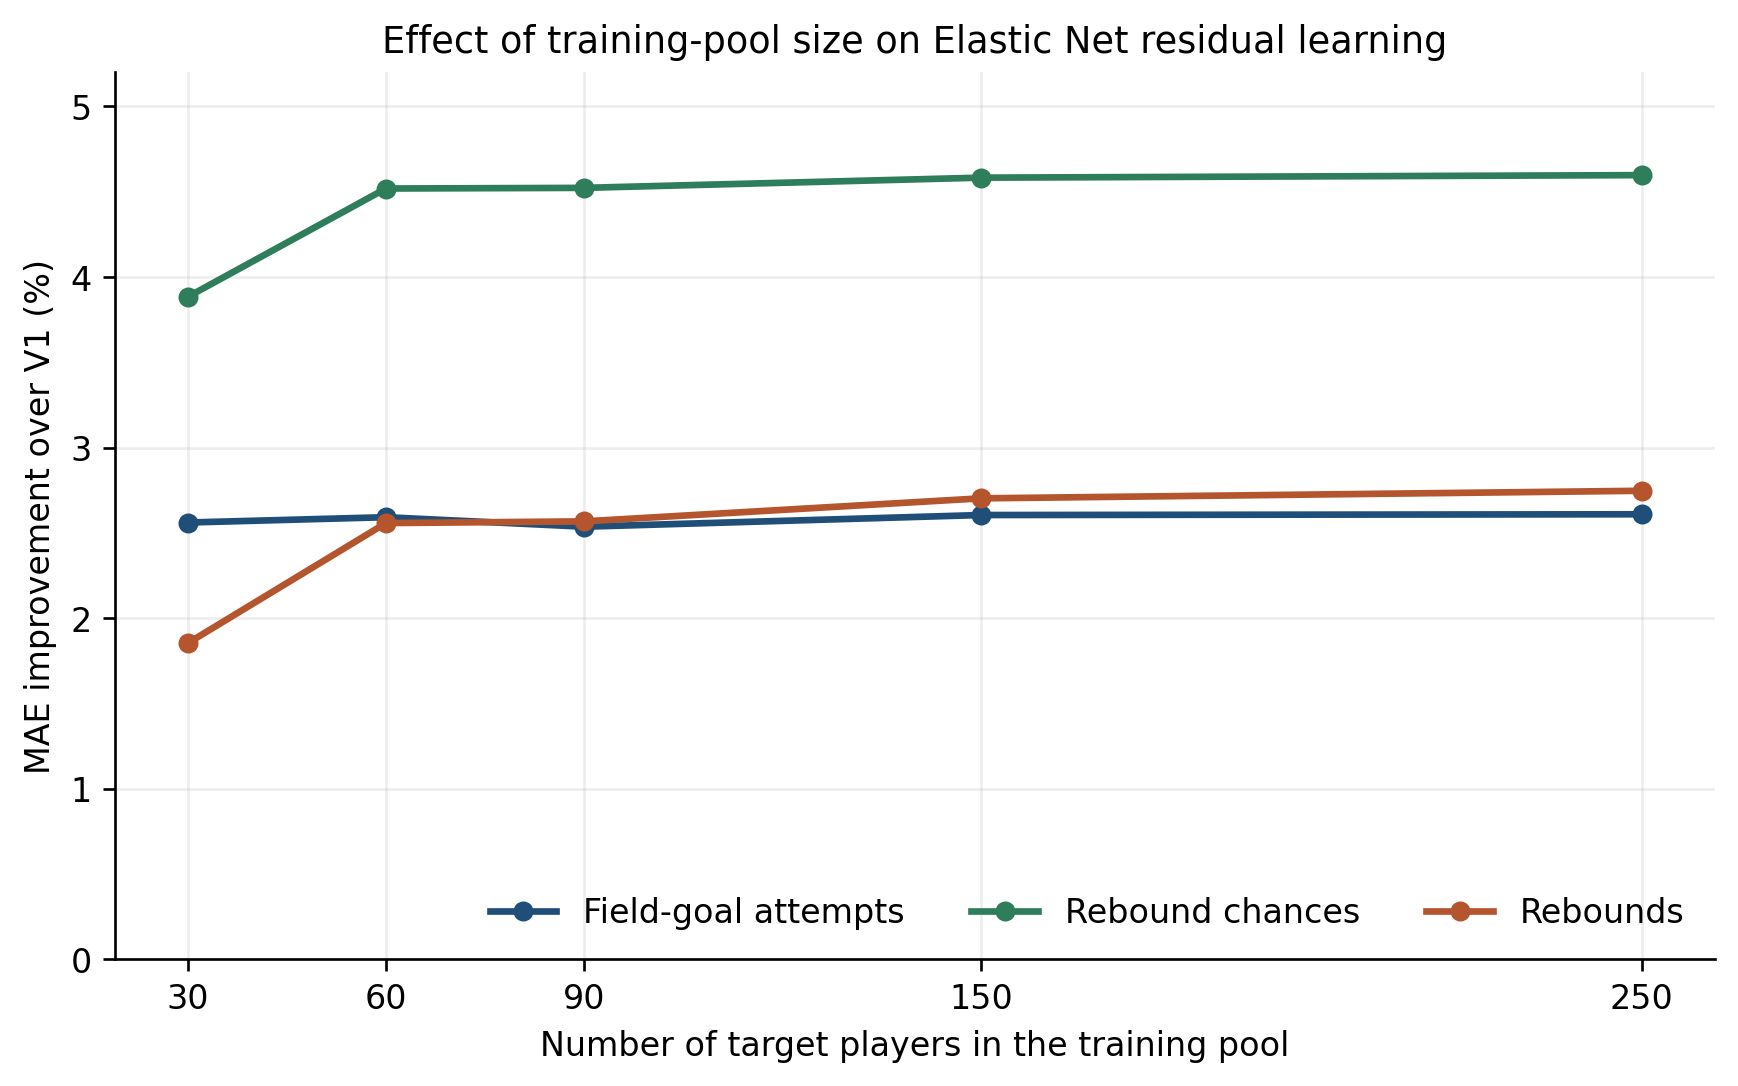
\includegraphics[draft=false,width=0.88\textwidth]{pool_size_learning_curve.png}
\caption{Learning curve for Elastic Net residual models on one common
chronologically later 2025--26 test set. The curves show diminishing returns
as the target-player training pool expands.}
\label{fig:pool-size}
\end{figure}
\newpage
Across the rolling outer seasons, the multitask MLP was slightly better on FGA
and rebounds but slightly worse on rebound chances. Its signed residuals were
highly correlated with those of Elastic Net, ranging from 0.94 to 1.00 across
outputs and approximately 0.97 when pooled. It also required substantially
more training time. Elastic Net was therefore selected because the small
average accuracy difference did not justify the neural model's additional
complexity and training cost.

\begin{table}[H]
\centering
\caption{Equal-season opportunity-model comparison across the three
chronologically held-out test seasons. Rebound estimates use the target's
recent conversion rate; learned conversion is evaluated separately in
Section~\ref{sec:conversion-results}.}
\label{tab:model-comparison}
\small
\begin{tabular}{llrrr}
\toprule
Model & Output & Mean V1 MAE & Mean V2 MAE & Improvement \\
\midrule
Elastic Net & FGA & 3.136 & 3.062 & 2.36\% \\
Elastic Net & Rebound chances & 3.063 & 2.934 & 4.22\% \\
Elastic Net & Rebounds & 2.122 & 2.066 & 2.64\% \\
Multitask MLP & FGA & 3.136 & 3.058 & 2.49\% \\
Multitask MLP & Rebound chances & 3.063 & 2.936 & 4.13\% \\
Multitask MLP & Rebounds & 2.122 & 2.065 & 2.70\% \\
\bottomrule
\end{tabular}
\end{table}

\subsection{Chronological outer-season performance}

The selected Elastic Net opportunity model improved all three outputs in each
of the three chronologically held-out test seasons. Figure~\ref{fig:outer-mae} shows the season-level
results, while Table~\ref{tab:model-comparison} reports equal-season means.

\begin{figure}[htbp]
\centering
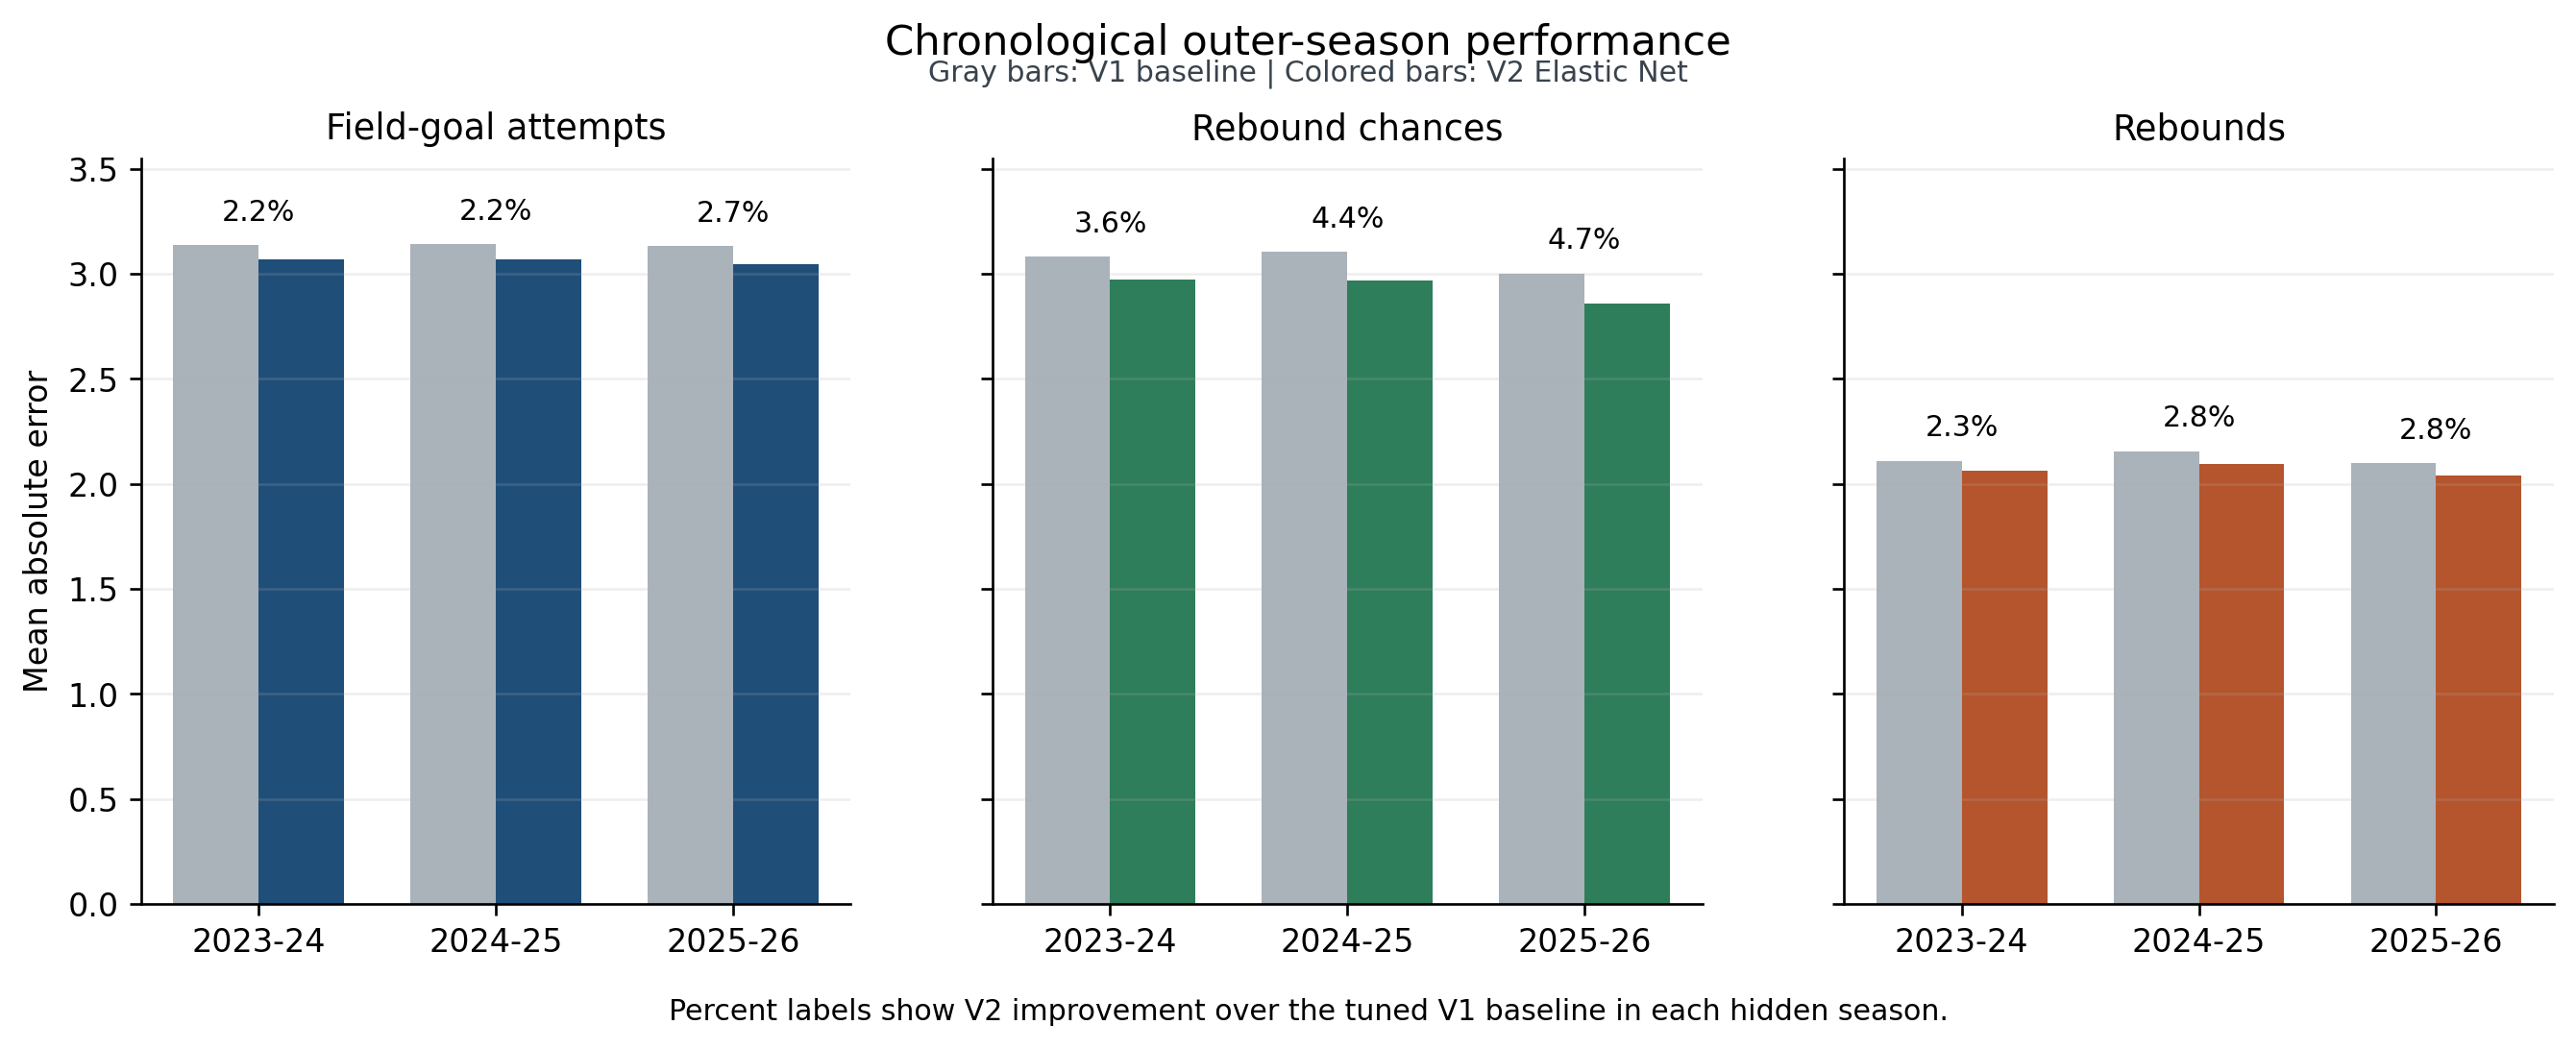
\includegraphics[width=\textwidth]{rolling_outer_season_mae.png}
\caption{V1 and Elastic Net V2 player-game-weighted MAE in each chronological outer
season. Axes begin at zero to avoid visually overstating the modest gains.}
\label{fig:outer-mae}
\end{figure}

The largest repeatable gain occurred for rebound chances, the opportunity
target most directly tied to the matchup and profile design. Rebound gains
were smaller because opportunity error is compounded by conversion variance.

\subsection{Normal-minutes experiment}

A game was labeled normal when actual minutes were close to the pregame
workload estimate. Here, $M_{expected}$ is the target player's mean minutes
across qualifying games in the recent baseline window. A game was considered
normal when

\[
|M_{actual}-M_{expected}|\leq
\max(3,0.15M_{expected}).
\]

Approximately 59\% of training and test rows met this condition. Evaluation
was restricted to normal-minute games, while training used either all games or
only normal-minute games.

\begin{table}[H]
\centering
\caption{Conditional MAE on normal-minute games.}
\label{tab:normal-minutes}
\small
\begin{tabular}{lrrr}
\toprule
Training cohort & FGA MAE & Rebound-chance MAE & Rebound MAE \\
\midrule
V1 reference & 2.819 & 2.764 & 2.014 \\
V2 trained on all games & 2.786 & 2.691 & 1.987 \\
V2 trained on normal-minute games & 2.767 & 2.680 & 1.988 \\
\bottomrule
\end{tabular}
\end{table}

The rebound values in Table~\ref{tab:normal-minutes} use the target's recent
conversion rate and precede the dedicated conversion experiment.

Normal-minute training modestly improved conditional FGA and rebound-chance
accuracy, while the initial rebound result was essentially unchanged. The normal-minutes model was retained alongside the all-games model as a
conditional projection. It estimates performance under the assumption that the player receives
approximately the expected workload; it cannot determine before the game
whether that condition will occur.

\subsection{Robust multiplier bounds}

The 0.50--1.50 interval affected fewer than 0.2\% of complete-season rows.
Average MAE and 99th-percentile absolute error changed only slightly, while the
largest observed rebound-chance and rebound errors were substantially reduced.
The bounds were therefore retained as protection against rare extreme matchup
ratios rather than as a source of average-accuracy improvement.

\begin{table}[H]
\centering
\caption{Effect of fixed 0.50--1.50 matchup bounds.}
\label{tab:bounds}
\small
\begin{tabularx}{\textwidth}{Xrr}
\toprule
Diagnostic & Unbounded & Bounded \\
\midrule
Mean FGA MAE & 3.062 & 3.062 \\
Mean rebound-chance MAE & 2.934 & 2.931 \\
Mean rebound MAE & 2.066 & 2.065 \\
Observed maximum rebound-chance absolute error & 55.847 & 22.412 \\
Observed maximum rebound absolute error & 30.224 & 20.426 \\
Mean FGA 99th-percentile absolute error & 11.369 & 11.353 \\
Mean rebound-chance 99th-percentile absolute error & 11.187 & 11.156 \\
Mean rebound 99th-percentile absolute error & 7.916 & 7.899 \\
FGA test rows clipped & 0\% & 0.134\% \\
Rebound-chance test rows clipped & 0\% & 0.186\% \\
\bottomrule
\end{tabularx}
\end{table}

The bounds are safety controls rather than filters. Raw ratios remain available
for audit and as machine-learning features.

\subsection{Rebound-conversion experiment}
\label{sec:conversion-results}

The recent player conversion rate was compared with position-prior shrinkage
and a chance-weighted Elastic Net correction while holding the corrected
rebound-chance forecast fixed.

\begin{table}[H]
\centering
\caption{Equal-season rebound MAE by conversion method.}
\label{tab:conversion}
\small
\begin{tabular}{lrrrr}
\toprule
Method & All games & Gain & Normal minutes & Gain \\
\midrule
Recent player rate & 2.0645 & -- & 1.9876 & -- \\
Position-prior shrinkage & 2.0506 & 0.68\% & 1.9662 & 1.08\% \\
Elastic Net adjustment & 2.0467 & 0.86\% & 1.9631 & 1.23\% \\
\bottomrule
\end{tabular}
\end{table}

All three chronologically held-out test seasons improved under the learned adjustment. For the
all-games setting, the mean reduction of 0.0179 rebounds had a
player-clustered 95\% bootstrap interval of approximately 0.0132 to 0.0225. In
the normal-minutes setting, the mean reduction of 0.0245 had an interval of
approximately 0.0189 to 0.0303. The effect is small in magnitude but repeatable.

\section{Discussion}

The strongest result is not a dramatic reduction in single-game error. It is
the consistency of the residual-model improvements across chronological test
seasons. Recent workload provides an interpretable starting point; per-minute
rates support player comparison; statistical similarity makes manual
comparison repeatable; and sample trust and bounds limit weak or extreme
opponent adjustments.

\begin{table}[H]
\centering
\caption{Interpretation of the five research hypotheses.}
\label{tab:hypotheses}
\small
\begin{tabularx}{\textwidth}{lXl}
\toprule
Hypothesis & Evidence & Assessment \\
\midrule
H1 & Recent stable-workload features formed a strong reference model, but a
separate season-wide comparison against every simpler averaging baseline was
not the focus of the final experiment. & Provisionally supported \\
H2 & Similar-player matchup evidence provided an auditable, bounded opponent
adjustment, but its incremental value over a neutral multiplier was not
isolated in the final outer folds. & Not directly tested \\
H3 & Elastic Net residual correction reduced MAE for all three outputs in all
three chronologically held-out test seasons. & Supported \\
H4 & Normal-minute training improved conditional FGA and rebound-chance MAE;
the first rebound comparison was flat, while learned conversion later improved
conditional rebounds. & Partially supported \\
H5 & Learned conversion reduced rebound MAE in every chronologically held-out test season, with
player-clustered bootstrap intervals above zero. & Supported \\
\bottomrule
\end{tabularx}
\end{table}

Typical errors remained near three FGA, three rebound chances, and two
rebounds. Important causes include unexpected playing time, injuries, foul
trouble, blowouts, teammate availability, role changes, opponent shot volume
and location, competition for the same rebound, imperfect player similarity,
and irreducible single-game variation. These errors should be understood as
the remaining uncertainty of a point forecast, not simply as a failure to fit
a more complex algorithm.

Elastic Net was selected as the final model because it retained the basketball
structure and matched the neural benchmark closely. The result is easier to
audit, faster to retrain, and less operationally demanding. This does not imply
that neural networks are generally unsuitable for basketball data; it means
that the tested tabular feature set did not contain enough additional nonlinear
signal to justify the more complex model.

\section{Limitations}

\begin{enumerate}
    \item \textbf{Minutes and availability.} Expected minutes are based on
    recent qualifying games. The model does not ingest timestamped injury
    reports, confirmed starters, restrictions, coach reports, or depth-chart
    changes.
    \item \textbf{Lineups and teammates.} Active-roster, lineup, on/off, and
    teammate-absence features are not represented, although they can sharply
    change usage and rebound role.
    \item \textbf{Opponent representation.} Opponent effects are inferred from
    comparable-player outcomes rather than explicit pace, shot-location mix,
    scheme, team rebounding, or expected game environment.
    \item \textbf{Similarity assumptions.} Weighted Euclidean distance is
    interpretable but imposes a simple geometry. Its weights were informed by
    basketball reasoning rather than optimized end to end.
    \item \textbf{Rebound-chance quality.} Total chances do not capture
    contested status, chance distance, offensive/defensive split, opponent shot
    profile, or teammate competition.
    \item \textbf{Point forecasts.} The system does not provide calibrated
    prediction intervals or threshold probabilities.
    \item \textbf{Scope.} Evidence is limited to regular-season tracking-era
    data and a reproducibly selected 250-player target pool. It does not
    establish playoff accuracy or future-season stability.
\end{enumerate}

\section{Conclusion and Future Work}

This project demonstrates that an interpretable basketball model and a modest
machine-learning correction can work together. The selected system reduced
average error relative to its tuned V1 reference in every chronological outer
season, reduced observed extreme errors through robust matchup bounds, and found
a small repeatable signal in rebound conversion. The gains are meaningful but
limited: the model improves a noisy single-game forecast rather than making it
certain.

The highest-priority extension is a pregame minutes and availability
model using timestamped injury status, confirmed starters, recent rotations,
return-from-injury indicators, and blowout risk. Further work should add
calibrated prediction intervals, lineup context, rebound-chance quality,
chronologically tuned similarity weights, and ongoing drift monitoring.

\begin{thebibliography}{9}

\bibitem{nbaapi}
\textit{nba\_api: An API Client Package to Access NBA.com APIs},
version 1.11.4.
GitHub repository and endpoint documentation.
\url{https://github.com/swar/nba_api}.
Accessed August 7, 2026.

\bibitem{nbaglossary}
National Basketball Association.
\textit{NBA Stats Help: Glossary}.
\url{https://www.nba.com/stats/help/glossary}.
Accessed August 7, 2026.

\bibitem{zouhastie}
H. Zou and T. Hastie.
Regularization and variable selection via the elastic net.
\textit{Journal of the Royal Statistical Society: Series B},
67(2):301--320, 2005.

\bibitem{scikitlearn}
F. Pedregosa et al.
Scikit-learn: Machine learning in Python.
\textit{Journal of Machine Learning Research}, 12:2825--2830, 2011.

\bibitem{pytorch}
A. Paszke et al.
PyTorch: An imperative style, high-performance deep learning library.
In \textit{Advances in Neural Information Processing Systems 32}, 2019.

\end{thebibliography}

\appendix
\section{Final Model Parameters and Feature Groups}
\label{app:parameters}

\subsection{Similarity weights}

\begin{table}[H]
\centering
\caption{Default numeric player-similarity weights.}
\begin{tabular}{lr}
\toprule
Feature & Weight \\
\midrule
Minutes & 1.00 \\
FGA per minute & 1.25 \\
Rebound chances per minute & 1.50 \\
Usage rate & 1.25 \\
Touches per minute & 1.25 \\
Starter rate & 0.75 \\
\bottomrule
\end{tabular}
\end{table}

The default position mismatch penalty is 0.35, the default comparison pool is
ten players, and a stricter optional setting can require the same starter flag.

\subsection{Trust and final model parameters}
The selected trust anchors were 0.45 at five samples, 0.65 at ten samples,
and 0.90 at fifteen or more samples. Smoothstep interpolation was used between
anchors, and matchup multipliers were bounded to 0.50--1.50 before trust was
applied. The selected final model parameters are:

\begin{table}[H]
\centering
\begin{tabular}{lr}
\toprule
Parameter & Value \\
\midrule
FGA Elastic Net $\alpha$ & 0.005 \\
FGA $l_1$ ratio & 1.00 \\
Rebound-chance Elastic Net $\alpha$ & 0.005 \\
Rebound-chance $l_1$ ratio & 0.25 \\
Multiplier bounds & 0.50--1.50 \\
Random state & 42 \\
All-games conversion $\alpha$ & 0.003 \\
All-games conversion $l_1$ ratio & 0.10 \\
Normal-minutes conversion $\alpha$ & 0.003 \\
Normal-minutes conversion $l_1$ ratio & 0.25 \\
\bottomrule
\end{tabular}
\end{table}

\subsection{V2 feature groups}

The opportunity residual models use 38 numeric features and listed position as
one categorical feature. Numeric features are organized into five groups:

\begin{table}[H]
\centering
\begin{tabular}{lr}
\toprule
Feature group & Numeric features \\
\midrule
Recent baseline and workload & 11 \\
Target role profile & 8 \\
Comparison-pool diagnostics & 7 \\
Opponent matchup evidence & 8 \\
V1 projections & 4 \\
\midrule
Total & 38 \\
\bottomrule
\end{tabular}
\end{table}

The complete machine-readable feature schema is defined in the source code and
recorded in locally generated model manifests.

\section{Reproducibility}

The accompanying public repository contains the source code, feature
definitions, NBA Stats endpoint documentation, automated tests, figures, and
documented commands for rebuilding the historical warehouse, training
datasets, experiments, model manifests, and fitted models. Raw NBA data,
generated experiment outputs, model manifests, and fitted model binaries are
not versioned in the repository.

Project repository:
\url{https://github.com/Keezey/nba-player-opportunity-forecasting}.

Rebuilding the historical warehouse depends on continued availability of the
NBA Stats endpoints and may require maintenance if their schemas or request
behavior change.

\end{document}
